\chapter*{Introduzione}
Negli ultimi anni, grazie all'avvento di nuove tecnologie nel settore delle reti wireless
e dei dispositivi mobili le reti wireless sono diventate una parte fondamentale
dell'infrastruttura delle telecomunicazioni. Ormai l'utente pretende che la qualit\`a
delle reti wireless siano almeno pari a quelli forniti via cavo visti gli incredibili passi avanti
che le reti cellulari hanno ottenuto negli ultimi 5-6 anni.
Basti pensare alla nuove reti 4G (LTE e WiMax) che promettono velocit\`a nell'ordine sui 5-8 Mbps
in download e contro le attuali linee ADSL con una media di 15 Mbps promessi.
In pi\`u le attuali societ\`a telefoniche forniscono pi\`u facilmente reti wireless ad alta velocit\`a
piuttosto che reti cablate vista la diffusione di apparecchiature mobili quali smartphone, tablet, e cos\`i via [Figura 1].
\begin{figure}
\begin{center}
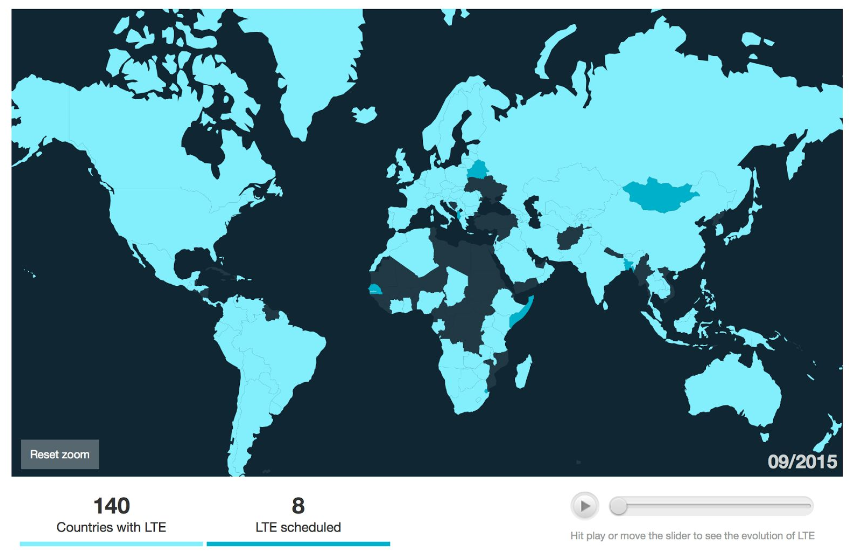
\includegraphics[scale=0.5]{LTE_Country_09_2015.png}
\caption[Cop LTE]{Copertura LTE mondiale}
\label{etichetta}
\end{center}
\end{figure}
In pi\`u con gli attuali progetti di Facebook e Google sulla progettazione di droni capaci di portare
reti WiFi o LTE si punta ad avere una copertura quasi totale del suolo mondiale.\\
Questa sempre pi\`u crescente utenza connessa in movimento ha fatto accrescere l'interesse di
acquisire informazioni contestuali per poter offrire servizi di maggior interesse e utilit\`a
per l'utente. L'informazione contestuale pu\`o riferirsi alla posizione dell'utente, all'ora attuale,
a propriet\`a fisiche come la temperatura, ecc.
La gestione efficiente del contesto richiede un dettagliato data modeling ottenuto
con processi specifici di classificazione, inferenza e predizione.\\
Certo \`e difficile comprendere cosa pu\`o essere considerato context aware,
senza prima avere dato una definizione di contesto. La principale definizione
di contesto \`e la seguente:
\textit{Il contesto \`e qualsiasi informazione che pu\`o essere usata per caratterizzare
la situazione di una entit\`a. Un' entit\`a e una persona, un luogo o un oggetto considerato rilevante all'interazione fra l'utente
e l' applicativo, inclusi l'utente e l'applicativo stessi}
\cite{cit_48}. Il contesto dunque \`e specificato
mediante i valori di opportuni parametri, rappresentanti l'attivit\`a di un'entit\`a
L'approccio orientato al contesto quindi permette all'entit\`a di adattarsi all'ambiente,
offrendo superiori vantaggi e possibilit\`a ai nuovi applicativi.\\
Una delle propriet\`a che maggiormente si desidera nel mobile context-awareness
\`e la possibilit\`a di poter effettuare previsioni, caratteristica che permetterebbe
lo sviluppo di nuove, avanzate applicazioni.\\
Nel 2001, il Computer Science and Telecommunications Board (CSTB) del
Consiglio Nazionale della Ricerca degli Stati Uniti d'America ha riunito una
commissione di esperti per eseguire una ricerca sulle opportunit\`a certe e sui
possibili sviluppi relativi all'interazione tra le comunit\`a di ricerca geo-spaziale
ed informatica. Nella relazione prodotta dalla commissione \cite{cit_47}, si evidenzia
come l'ubicazione dell'utente sia uno dei fattori fondamentali nelle diverse
definizioni di contesto che sono state proposte in letteratura. La centralit\`a
di tale componente e la possibilit\`a, fornita dalle attuali tecnologie mobili, di
rilevare in modo sufficientemente preciso, semplice e continuativo, la posizione
geografica degli utenti, fanno di questo settore un campo di ricerca attualmente
molto attivo.\\
Contemporaneamente alla nascita dei servizi context aware, \`e dunque nata
la necessit\`a di avviare una ricerca mirata al miglioramento delle prestazioni
nella previsione delle traiettorie. Tale ramo di ricerca ovviamente mutua gran
parte della natura delle applicazioni context aware. In questo caso per\`o le
informazioni memorizzate si riducono a semplici dati spaziali e temporali, che
possono ledere la privacy della persona in minima parte, ma non in modo cos\`i
invasivo come, invece, possono essere portati a fare con applicativi context aware,
che per loro natura cercano di tracciare tutti gli aspetti (gusti, personalit\`a)
dell'utenza. La conoscenza della posizione di oggetti mobili ha dunque condotto
allo sviluppo di applicazioni e servizi che sono stati catalogati location-based,
che necessitano di conoscere la posizione approssimata di un oggetto mobile per
operare. Esempio di tali servizi sono gli applicativi di navigazione, gestori
di traffico e la pubblicit\`a location-based. In uno scenario tipico, il
dispositivo mobile che sta fornendo un determinato servizio, periodicamente
informa il framework di posizionamento della attuale posizione.\\
Nell'ultimo decennio anche i sistemi di sistemi di posizionamento sono migliorati.
da un'accuratezza di decine di metri, si \`e ormai arrivati ad avere una precisione
di pochi metri anche per utilizzi civili. La ricerca di una precisione sempre
pi\`u alta a disposizione di tutti ha portato alla creazione di sistemi di posizionamento
alternativi al GPS quali GLONASS (Militare russo), COMPASS (Cina), Galileo (Europa) e IRNSS (India)
stanno cercando di imporsi come alternativa al sistema Americano.\\
Grazie alla copertura sempre crescente di reti wireless e sistemi di posizionamento la
context aware non \`e pi\`u incentrata sulla ricerca della posizione attuale dell'utente, ma sulle possibili destinazioni
e percorsi nel breve e lungo termine. Grazie ad una metodologia si cerca di predire la posizione
per anticipare i movimenti dell'utente e quindi cercare di eseguire un pre-fetch
del servizio sulla localit\`a prevista.
Lo sviluppo di pratiche ed accurate tecniche di previsione degli spostamenti
pu\`o dunque aprire le porte a molti applicativi quali prenotazione di risorse,
servizi location-based, ma anche migliorare la pianificazione e gestione delle
aree urbane, grazie ad una migliore analisi del flusso urbano.\\
Ovviamente la possibilit\`a di tracciare la posizione attuale dell'utente da sola non \`e sufficiente
ad effettuare previsioni sul futuro dell'utente. In un articolo pubblicato qualche anno fa
 \cite{new_1}, nel quale si afferma come osservando i dati storici relativi ai movimenti di un utente
(collezionati con diverse tecniche, nel caso citato accedendo alle basi di dati di una compagnia telefonica)
sia possibile individuare pattern di movimento, e prevedere correttamente il luogo in cui
si trova una persona per il 93\% del tempo. Da tali studi emerge come ciascun
individuo abbia un insieme di localit\`a che raramente lascia, e nelle quali si
sposta con grande regolarit\`a. Gli utenti che risiedono stabilmente in un raggio
di 6 miglia hanno un tasso di predicibilit\`a della posizione che va dal 93\% al
97\%, ma anche nel caso in cui il raggio aumenti di centinaia di miglia, la
percentuale delle previsioni rimane alta, stabilizzandosi al 93\% di successo.
In tale articolo vengono inoltre indicati dei legami tra le localit\`a frequentate
dall'individuo e le ore della giornata. In particolare si evince come in
certi orari di transizione (prima o dopo l'orario di lavoro, oppure durante le
pause pranzo) le previsioni sul luogo in cui si trova l'utente vedano un brusco
peggioramento dei risultati; comunque la percentuale che l'utente si trovi in
un qualsiasi momento della giornata nella localit\`a pi\`u visitata \`e molto alta (del
70\%).

\section{Obiettivi della tesi}
Gi\`a in precedenti lavori di tesi svoltesi nell'Universit\`a degli Studi di Udine \`e
stato presentato un algoritmo di previsione delle traiettorie basato sul modello
della fisica dei campi elettrici, dove le localit\`a maggiormente importanti
per l'individuo erano caratterizzate da forze attrattive e le meno importanti
da forze nulle se non addirittura repulsive. Tale algoritmo \`e denominato
ARDA, \`e stato presentato unitamente ad una nuova proposta di pesatura dell'importanza
delle localit\`a che prende il nome di SpaceRank, il quale andava
ad affiancare altri indici di valutazione delle localit\`a quali TotalTime (il tempo
totale che l'individuo passa in una localit\`a), AverageTime (il tempo medio che
l'individuo passa in una certa localit\`a durante una visita), NumberOfVisits (il
numero di volte che l'utente passa per una certa localit\`a), e combinazioni di
tali indici.
Il lavoro svolto in una precedente tesi \cite{new_1} proponeva:
\begin{itemize}
\item L'implementazione dell'algoritmo di previsione ARDA utilizzando vari indici di valutazione
dell'importanza delle localit\`a, con diverse suddivisioni di territorio

\item Il confronto dei risultati di previsione ottenuti evidenziando il comportamento
dell'algoritmo ARDA rispetto a due altri algoritmi di previsione( il primo
che suppone l'utente prosegua la propria corsa in linea retta mantenendo la
velocit\`a media, il secondo che suppone l'utente prosegua il proprio percorso
rimanendo in un intorno del punto rilevato);

\item La valutazione di stabilit\`a degli algoritmi proposti eseguendo dei test anche su una diversa raccolta di punti GPS (messa a disposizione
dal Prof. Thad Starner) riguardante un territorio di dimensioni e variet\`a di movimenti maggiori;

\item L'analisi del comportamento dell'algoritmo nelle previsioni delle destinazioni finali, eseguite
lungo quattro milestone virtuali poste lungo i percorsi (inizio, 25\%, 50\% e 75\% del tracciato).

\end{itemize}

Questa tesi prende in esame l'algoritmo e i dati di quella precedentemente descritta e si pone i seguenti obbiettivi:
\begin{itemize}
\item Traduzione degli algoritmi dal linguaggio Python a Java e miglioramento di alcuni aspetti;
\item Unificazione delle procedure di test per i vari indici;
\item Sviluppo di un'interfaccia per l'utilizzo al di fuori della riga di comando;
\item Sviluppo di un sistema di visualizzazione ed esportazione dei test eseguiti.
\end{itemize}

\section{Struttura della tesi}
Lo scritto della tesi si divide in tre parti.
La prima parte si occupa di presentare gli algoritmi presi in esame cercando di metterne in evidenza
non solo gli aspetti modellistici, ma anche i problemi implementativi.
Nella seconda parte si d\`a ampio spazio ai risultati ottenuti sia nei risultati che a livelli
prestazionali.
Infine la terza parte \'e quella conclusiva, in cui si riassume il lavoro svolto traendone
le somme, presentando i punti di forza e di debolezza delle soluzioni
adottate dando anche degli spunti di riflessione su eventuali sviluppi.\\

Le tre parti sopra esposte in realt\`a sono state svolte con diversa estensione,
cercando di rispettare le gerarchie logiche.
La prima sezione \'e racchiusa nei capitoli 1 e 2.
Il primo capitolo espone i concetti e la teoria sugli algoritmi scelti (prendendo spunto
dalla tesi \cite{cit_49}), vista l'importanza di riuscire a proporre nel
modo pi\`u esauriente possibile le soluzioni algoritmiche adottate. Il secondo
capitolo invece si sofferma sulle scelte di sviluppo fatte, gli accorgimenti
fatti per migliorare gli algoritmi e il funzionamento del programma.
La seconda parte invece si sviluppa nei seguenti due capitoli.
Nel terzo capitolo si espongono i risultati ottenuti comparandoli con quelli
della tesi precedente lasciando spazio a grafici e confronti cercando
di capire il perch\'e delle differenze.
Nel quarto capitolo si fa una piccola osservazione sulle prestazioni delle 2 versioni
facendo anche un confronto con i tempi stimati al tempo della tesi originale.
Infine la terza parte, quella conclusiva, nella quale si cerca con il quinto capitolo
di riassumere il lavoro svolto, evidenziando i risultati ottenuti e cercando
di proporre come poter ulteriormente sviluppare la ricerca e migliorarne le prestazioni.
